\documentclass[12pt]{article}

% a template that a friend gave, it's worked well enough for me
% i have added some packages and stuff that have proved useful

\usepackage{fancyhdr}
\usepackage{tipa}
\usepackage{fontspec}
\usepackage{amsfonts}
\usepackage{enumitem}
\usepackage[margin=1in]{geometry}
\usepackage{graphicx}
\usepackage{float}
\usepackage{amsmath}
\usepackage{braket}
\usepackage{amssymb}
\usepackage{booktabs}
\usepackage{hyperref}
\usepackage{mathtools}
\usepackage{xcolor}
\usepackage{float}
\usepackage{algpseudocodex}
\usepackage{titlesec}
\usepackage{bbm}

\pagestyle{fancy}
\fancyhf{} % sets both header and footer to nothing
\lhead{Kevin Sheng}
\setmainfont{Comic Neue}
\renewcommand{\headrulewidth}{1pt}
\setlength{\headheight}{0.75in}
\setlength{\oddsidemargin}{0in}
\setlength{\evensidemargin}{0in}
\setlength{\voffset}{-.5in}
\setlength{\headsep}{10pt}
\setlength{\textwidth}{6.5in}
\setlength{\headwidth}{6.5in}
\setlength{\textheight}{8in}
\renewcommand{\headrulewidth}{0.5pt}
\renewcommand{\footrulewidth}{0.3pt}
\setlength{\textwidth}{6.5in}
\usepackage{setspace}
\usepackage{multicol}
\usepackage{float}
\setlength{\columnsep}{1cm}
\setlength\parindent{24pt}
\usepackage [english]{babel}
\usepackage [autostyle, english = american]{csquotes}
\MakeOuterQuote{"}

\setlength{\parskip}{6pt}
\setlength{\parindent}{0pt}

\titlespacing\section{0pt}{12pt plus 4pt minus 2pt}{0pt plus 2pt minus 2pt}
\titlespacing\subsection{0pt}{12pt plus 4pt minus 2pt}{0pt plus 2pt minus 2pt}
\titlespacing\subsubsection{0pt}{12pt plus 4pt minus 2pt}{0pt plus 2pt minus 2pt}

\hypersetup{colorlinks=true, urlcolor=blue}

\newcommand{\correction}[1]{\textcolor{red}{#1}}


\begin{document}
\begin{enumerate}
    \item \begin{align*}
              \frac{\partial}{\partial y} (1-y\sin x) & =-\sin x & \frac{\partial}{\partial x} \cos x & = -\sin x
          \end{align*}
          Since these two are equivalent, this equation is exact.
          \begin{gather*}
              \int (1-y\sin x)\,dx =x+y \cos x +f(y) \\
              \int \cos x\,dy=y \cos x+g(x)
          \end{gather*}
          Combining these two equations together gives us $\boxed{x+y \cos x=C}$.
    \item Taking the differentials for this one, we have:
          \begin{align*}
              \frac{\partial}{\partial y} (y^2-xy) & =2y-x & \frac{\partial}{\partial x} x^2 & = 2x
          \end{align*}
          This equation as it is is not exact, since the two partials differ.
          After multiplying both sides by $u(x)=\frac{1}{xy^2}$, we get the following:
          \begin{align*}
              \frac{\partial}{\partial y} \frac{1}{x}-\frac{1}{y} & =\frac{1}{y^2}
                                                                  & \frac{\partial}{\partial x} \frac{x}{y^2} & = \frac{1}{y^2}
          \end{align*}
          These two are equal, so we can go ahead and solve the equation now.
          \begin{gather*}
              \int \frac{1}{x}-\frac{1}{y}\,dx=\ln |x| - \frac{x}{y}+f(y) \\
              \int \frac{x}{y^2}\,dy=-\frac{x}{y}+g(x) \\
              \boxed{\ln |x|-\frac{x}{y}=C}
          \end{gather*}
    \item We have to check if the RHS and its partial wrt $\omega$ is continuous on the region defined by the initial conditions.
          The RHS by itself is continuous everywhere, so this isn't a problem.
          As for its partial, we have \[\frac{\partial}{\partial \omega} \omega \sin \omega +s=\omega \cos \omega+\sin \omega\]
          which is also continuous everywhere.
          Thus, we're guaranteed a unique solution.
    \item Checking the solutions wrt the diffeq, we have
          \begin{gather*}
              y(t)=0 \rightarrow y'(t)=0 \rightarrow 0=3(0)^{2/3} \\
              y(t)=t^3 \rightarrow y'(t)=3t^2 \rightarrow 3t^2=3(t^3)^{2/3}
          \end{gather*}
          It is evident that both of these equations are valid.
          Checking the initial conditions, we also have that $0=0$ and $0=0^3$, so those don't fail either.

          This does not contradict the uniquenesss theorem because the derivative
          of the RHS wrt $y$, $2(y)^{-1/3}$, is not continuous at the given initial conditions.
    \item The given differential equation is not exact.
    \begin{gather*}
        \frac{\partial}{\partial y} \left(-2 \sin \left(x^2\right)+2y^2\right)=y^4 \\
        \frac{\partial}{\partial x} 2xy=2y
    \end{gather*}
    To make it exact, we multiply both sides by some $u(x)$.
    For this to work, $u(x)$ has to satisfy
    \[\frac{\partial}{\partial y}(u(x)\left(-2\sin \left(x^2\right) +2y^2\right))=\frac{\partial}{\partial x} (u(x) 2xy)\]
    After expanding the derivatives, we get
    \[u(x) \cdot 4y= u(x) \cdot 2y+ 2xy \cdot u'(x)\]
    This then simplifies to $u(x)=x \cdot u'(x)$ which means $u(x)=x$.

    Now we have $P(x,y)=-2x\sin\left(x^2\right)+2xy^2$ and $Q(x,y)=2x^2y$.
    Integrating, we have
    \begin{gather*}
        \int -2x\sin\left(x^2\right)+2xy^2\,dx=x^2y^2+\cos\left(x^2\right)+f(y) \\
        \int 2x^2y\,dy=xx^2y^2+g(x)
    \end{gather*}
    which gives us the \textit{implicit} solution $x^2y^2+\cos\left(x^2\right)=C$.

    Next we plug in the initial condition $y(\sqrt \pi)=1$.
    $\pi \cdot 1+ \cos \pi=C$, which gives us $C=\pi-1$.
    Also, since we need the explicit solution, we isolate $y$ to get
    \[\boxed{y=\frac{\sqrt{\pi-1-\cos x^2}}{x}}\]
    \item The solutions to the polynomial $y(y^2-1)$ are $0$, $1$, and $-1$.

    Taking the derivative of this gives us $3y^2-1$, and plugging the solutions we obtained into it gives us the following results:
    \begin{itemize}
        \item $0$: $3 \cdot 0^2-1<0 \rightarrow$ stable
        \item $1$: $3 \cdot 1^2-1>0 \rightarrow$ unstable
        \item $-1$: $3 \cdot (-1)^2-1>0 \rightarrow$ unstable
    \end{itemize}
    \begin{center}
        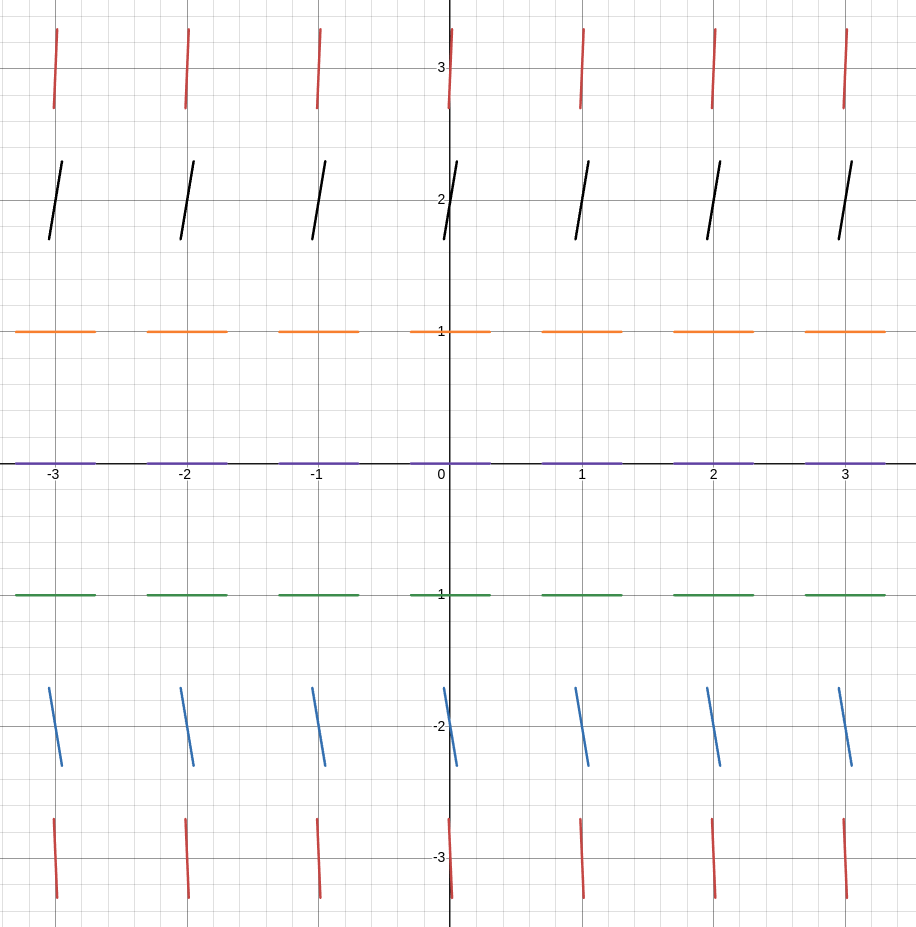
\includegraphics[width=8cm]{img/slope_field} \\
        \small{The slope field of this equation. \\ Notice the horizontal lines at all the $y$-values specified above.}
    \end{center}
\end{enumerate}
\end{document}
